\documentclass[10pt,mathserif]{beamer}
\usepackage[T5]{fontenc}
\usepackage{fontspec}
\setsansfont{Segoe UI}
%\setmainfont{Segoe UI}
\usepackage[utf8]{inputenc}
% Style
\usepackage{graphicx,amsmath,amssymb,tikz,psfrag,amsthm,enumerate}
\usepackage[backend=biber,style=numeric,citestyle=ieee]{biblatex}
%\usepackage[backend=biber,style=authoryear,citestyle=ieee]{biblatex}

\addbibresource{references.bib}

% ~~~~~~~~~~~
% References
%\addbibresource{references.bib}


%********************* Custom  *********************  


% Chèn và định dạng mã nguồn
\usepackage{listings}
\usepackage{color}


% Chèn và định dạng mã giả
\usepackage{amsmath}
\usepackage{algorithm}
\usepackage[noend]{algpseudocode}
\makeatletter
\def\BState{\State\hskip-\ALG@thistlm}
\makeatother

% Bảng biểu
\usepackage{multirow}
\usepackage{array}
\newcolumntype{L}[1]{>{\raggedright\let\newline\\\arraybackslash\hspace{0pt}}m{#1}}
\newcolumntype{C}[1]{>{\centering\let\newline\\\arraybackslash\hspace{0pt}}m{#1}}
\newcolumntype{R}[1]{>{\raggedleft\let\newline\\\arraybackslash\hspace{0pt}}m{#1}}



% Vẽ cây
\usepackage{tikz}
\usetikzlibrary{calc}
\usetikzlibrary{trees}

% Dãn dòng 1.5
\usepackage{setspace}
\onehalfspacing

% Thụt vào đầu dòng
\usepackage{indentfirst}

% Canh lề
\usepackage[
top=30mm,
bottom=25mm,
left=30mm,
right=20mm,
includefoot]{geometry}

% Trang bìa
\usepackage{tikz}
\usetikzlibrary{calc}
\newcommand\HRule{\rule{\textwidth}{1pt}}
% ========================================================================================= %
% PACKAGE CUSTOMIZE
% pdf
\usepackage{pdfpages}

\usepackage[strings]{underscore}
\usepackage{url}

% Math
\usepackage{amsfonts}

\usepackage{stmaryrd}


% Vẽ cây
\usetikzlibrary{trees}

% caption
\usepackage[justification=centering,font=small,labelfont=bf]{caption}
\captionsetup[figure]{font=small}
% % subfigure
\usepackage[font=small,labelfont=bf]{subcaption}
\usepackage{wrapfig}
% \usepackage[justification=centering,font=normalsize]{caption}


\usepackage{tocloft}
\usepackage{tabularx}
\usepackage{booktabs}

% Bảng thuật ngữ
\usepackage[acronym,nomain]{glossaries}

% Customize 
\usepackage[export]{adjustbox}

\usepackage{multicol}

\graphicspath{{images/}}


% ~~~~~~~~~~~~ Custom ~~~~~~~~~~~~
%\usepackage{framed}
\usepackage[capitalise]{cleveref}
\usepackage{algorithm,algorithmicx,algpseudocode}
\usepackage{array}
\usepackage[parfill]{parskip}
%\usepackage{subcaption}
\usepackage{bm}
\usepackage{gensymb}
\usepackage[]{units}
\usepackage{listings}
\usepackage{multicol}
\usepackage{tcolorbox}
% -- \usepackage{physics}
\usepackage{ulem}
% ~~~~~~~~~~~~ Custom ~~~~~~~~~~~~
\graphicspath{{images/}}
\usepackage{hyperref}

\input{preamble/commands.tex}
% \logo{\includegraphics[height=0.6cm]{hcmus}}
% ~~~~~~~~~~~~ Custom ~~~~~~~~~~~~

%% formatting
\mode<presentation>
{
\usetheme{default}
%\usetheme{Berlin}
%\usetheme{Stanford}
\useinnertheme{circles}
}
\setbeamertemplate{navigation symbols}{}
\usecolortheme[rgb={0.13,0.28,0.59}]{structure}
%\setbeamertemplate{itemize subitem}{--}
\setbeamertemplate{frametitle} {
	\begin{center}
	  {\large\bf \insertframetitle}
	\end{center}
}

\newcommand\footlineon{
  \setbeamertemplate{footline} {
    \begin{beamercolorbox}[ht=2.5ex,dp=1.125ex,leftskip=.8cm,rightskip=.6cm]{structure}
      \footnotesize \insertsection
      \hfill
      {\insertframenumber}
    \end{beamercolorbox}
    \vskip 0.45cm	
  }
}
\footlineon

\AtBeginSection[] 
{ 
	\begin{frame}<beamer> 
		\frametitle{Outline} 
		\tableofcontents[currentsection,currentsubsection] 
	\end{frame} 
} 

\title{\large \bfseries OpenHuman: Sinh cử chỉ dựa trên âm thanh}
\subtitle{The synthesis system for conversational gestures based on emotion and semantics}

\include{preamble/meta.tex}
% ~~~~~~~~~~~~~~~~~~~~~~~~~~~~~~~~~~~~~~~~
\begin{document}

%\begin{frame}[plain]
%	\titlepage
%\end{frame}


%\include{sections/0.demo.tex}

%\section{Giới thiệu}

\begin{frame}{Động lực nghiên cứu}
	\vspace{5pt}
	
	\begin{columns}
	% Left column
	\begin{column}{0.7\textwidth}
		\textbf{Text-base Deep Learning}
		\begin{itemize}
			\item ChatGPT, Alexa, Character.AI,..
			\item Text to speech, text to text,..
		\end{itemize}
		
		\textbf{Text/audio to Realistic Digital Humam}
		
		\begin{itemize}
			\item Video-base (HeyGen, Midjourney,...)
			\item Rendering-base:
			\begin{itemize}
				\item Character model (Gaussian Splatting)
				\item Character animation: (3D keypoints)
			\end{itemize}
		\end{itemize}
		\vspace{5pt}
		\centering
		\includegraphics[width=0.8\textwidth]{FacialAsset.png}
	\end{column}
	
	% Right column
	\begin{column}{0.3\textwidth}
		\begin{figure}
				\includegraphics[width=\textwidth]{UniversalHuman.png}
%				\caption{\small Minh hoạ người kỹ thuật số siêu thật (realistic digital human)}
		\end{figure}
		
		\begin{figure}
			\includegraphics[width=\textwidth]{MetaHuman.jpg}
			\caption{\small Minh hoạ người kỹ thuật số siêu thật (realistic digital human)}
		\end{figure}
	
	\end{column}
	
	\end{columns}
\end{frame}



\begin{frame}{Dữ liệu bài toán}
	
	
	\begin{columns}
		
		\begin{column}{0.7\textwidth}
			
			\textbf{Dữ liệu}
			\begin{itemize}
				\item Dữ liệu chuyển động thu nhận từ cảm biến.
				\item Âm thanh tương ứng với cử chỉ.
			\end{itemize}
			
			\textbf{Kiến trúc khung xương}
			\begin{itemize}
				\item Chuỗi chuyển động khung xương $60 \text{fps}$
				\begin{itemize}
					\item Skeleton: 75 bones: $\mathbf{B} = \{ \mathbf{b}_i \}^{75} $ \\
					\small{(\texttt{Head}, \texttt{Spine}, \texttt{Hips}, \texttt{LeftArm},\texttt{RightArm}... )} \\
					Dữ liệu BVH: $\mathbf{b}_{i} = \{r_x, r_y, r_z\}$
				\end{itemize}
				\begin{figure}[h]
					\centering
					\includegraphics[width=0.9\textwidth]{BoneRotationSeries}
				\end{figure}
				
				\item Dữ liệu sau xử lý: $\mathbf{g} \in \mathbb{R}^{D}$, với $D=1141$ 
				$\mathbf{g} = \Big[ \mathbf{p},  \mathbf{r},
				\mathbf{ p }',  \mathbf{r}',
				\mathbf{p}_{\text{joins}},  \mathbf{r}_{\text{joins}},
				\mathbf{p}'_{\text{joins}},  \mathbf{r}'_{\text{joins}},
				\mathbf{d}_{\text{gaze}}
				\Big]$
			\end{itemize}
			\vspace{10pt}
%			\textbf{Loại bài toán}: Hồi quy (regression)
%			\begin{itemize}
%				\item Cho trước $N$ khung hình (frame) cử chỉ, dự đoán $M$ khung hình tiếp theo tương ứng với âm thanh $\mathbf{a}$.
%			\end{itemize}
		
		\end{column}
		
			\begin{column}{0.3\textwidth}
				\begin{figure}[h]
					\centering
					\includegraphics[width=\textwidth]{Skeleton}
				\end{figure}
		\end{column}
		
	\end{columns}
	
\end{frame}

\begin{frame}{Chuyển động của toạ độ}
		\begin{figure}
		\centering
		\includegraphics[width=\textwidth, height=40pt]{MotionXYZ.png}
		\caption{Minh hoạ chuyển động của góc quay một Bone trong toạ độ}
	\end{figure}
	
	\begin{columns}
		\begin{column}{0.8\textwidth}
			\begin{itemize}
				\item $\mathbf{p} \in \mathbb{R}^3$: Toạ độ của điểm gốc
				\item $\mathbf{r} \in \mathbb{R}^4$: Góc quay của điểm gốc
				\item $\mathbf{p}'_{\text{root}} \in \mathbb{R}^3$: Vận tốc thay đổi của toạ độ gốc
				\item $\mathbf{r}'_{\text{root}} \in \mathbb{R}^3$: Vận tốc thay đổi của góc quay gốc
				
				\item $\mathbf{p}_{\text{joins}} \in \mathbb{R}^{3 n_{\text{join} }}$: Toạ độ của các khung xương
				\item $\mathbf{r}_{\text{joins}} \in \mathbb{R}^{3 n_{\text{join} }}$: Góc quay của các khung xương
				\item $\mathbf{p}'_{\text{joins}} \in \mathbb{R}^{3n_{\text{join} }}$: Vận tốc thay đổi của toạ độ các khung xương
				\item $\mathbf{r}'_{\text{joins}} \in \mathbb{R}^{3n_{\text{join} }}$: Vận tốc thay đổi của góc quay các khung xương
				
				\item $\mathbf{d}_{\text{gaze}} \in \mathbb{R}^3$: Là hướng nhìn
			\end{itemize}
		\end{column}
		
		\begin{column}{0.2\textwidth}
			image here
			
		\end{column}
	\end{columns}
	
\end{frame}

\begin{frame}{Phát biểu bài toán}
%\frametitle{Group lasso \\[-0.3em] 
%{\footnotesize \textmd{(\eg, Yuan \& Lin; Meier, van de Geer, B\"uhlmann; Jacob, Obozinski, Vert)}}}


 \begin{figure}[h]
	\centering
	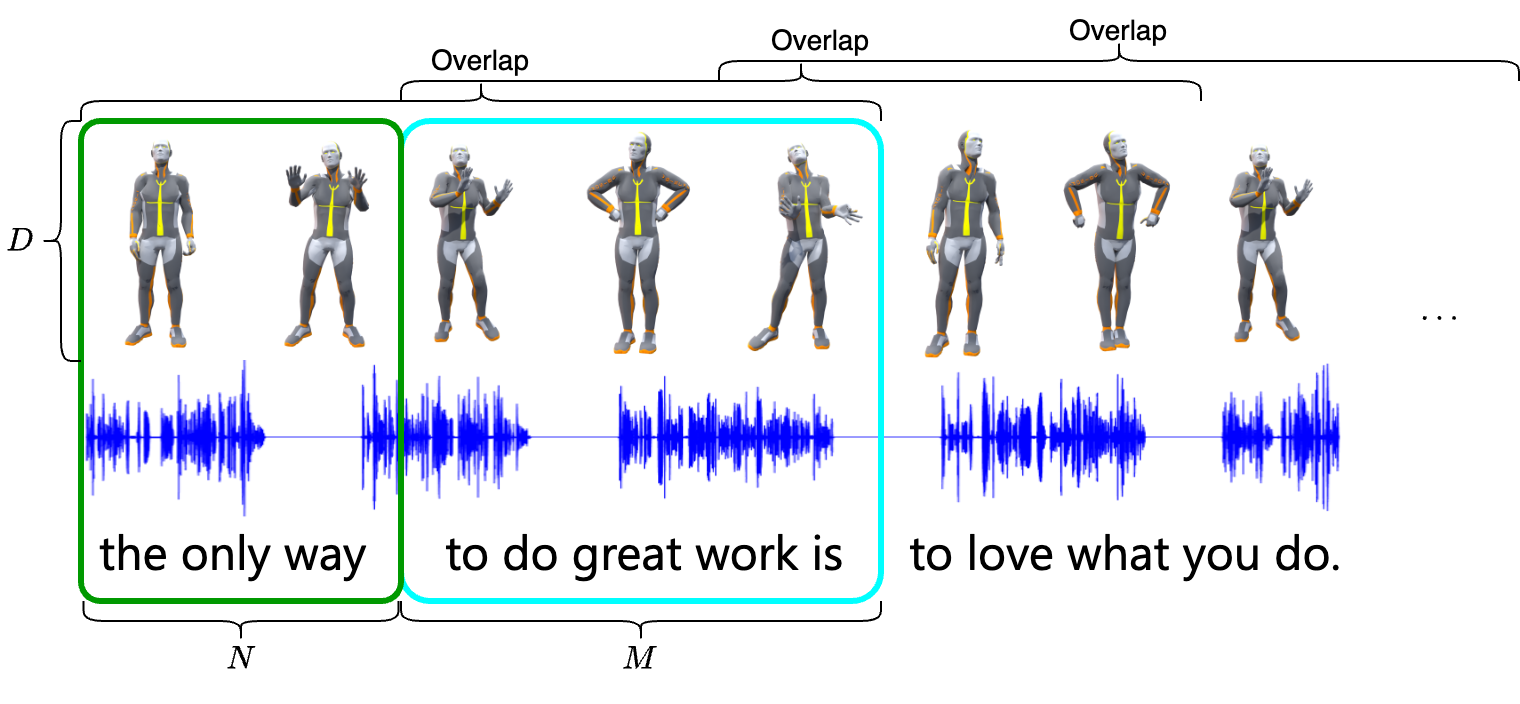
\includegraphics[height=4.5cm]{GestureSeries}
\end{figure}

\vspace{-10pt}

\begin{columns}
	
	\begin{column}{0.6\textwidth}
		
		\textbf{Input}
		\begin{itemize}
			\item Chuỗi cử chỉ khởi tạo: $\mathbf{s} \in \mathbb{R}^{N \times D}$
			\item Chuỗi âm thanh: $\mathbf{a}^{length}$ sample rate 16000 được cắt thành từng đoạn 4s: $\mathbf{a} \in \mathbb{R}^{6400}$
%			trích xuất đặc trưng MFCC: $\mathbf{a} \in \mathbb{R}^{M \times C_{\text{mfcc}}}$
			\item Cảm xúc: $\mathbf{e} \in \mathbb{R}^6$ (\texttt{Happy},  \texttt{Sad},  \texttt{Neutral}, \texttt{Angry}, \texttt{Old}, \texttt{Funny})
		\end{itemize}
		
	\end{column}
	\begin{column}{0.4\textwidth}
		 \textbf{Output}
		 \begin{itemize}
		 	\item Chuỗi cử chỉ dự đoán: $\hat{\mathbf{x}} \in \mathbb{R}^{M \times D}$
		 \end{itemize}
		 
		 \textbf{Grouth Truth}
		 \begin{itemize}
		 	\item Chuỗi cử chỉ gốc: $ \mathbf{x}  \in \mathbb{R}^{M \times D}$
		 \end{itemize}
	\end{column}
\end{columns}

\end{frame}

\begin{frame}{Khung chương trình}
	Sử dụng mô hình Diffusion Classifier-Free Guidance (có điều kiện) với cử chỉ $\bx^{1:M \times D}$ làm $x_0$ và điều kiện $c = [{\mathbf{s}, \mathbf{a}, \mathbf{e}}]$. $N = 8$, $M = 80 \sim \text{4 giây}$
%	$N=8$ khung hình đầu làm khởi tạo và $M=80$ khung hình để dự đoán
		\begin{figure}[h]
			\centering
			\includegraphics[width=\textwidth]{Framework}
		\end{figure}
	
%\textbf{Training}
%	\begin{itemize}
%		\item $f_{\theta}(\mathbf{g}_0, \mathbf{a}, \mathbf{e})$
%	\end{itemize}
%
%\textbf{Inference}
%
%	\begin{itemize}
%		\item $\mathbf{x}' = f_{\theta'}$
%	\end{itemize}
%Dữ liệu phải được chuẩn hoá trên toàn bộ tập dữ liệu với $\mu(g) = 0$ và $\sigma = 1$. $\bx_{i} = \frac{\bx_{i} - \mu}{\sigma}$.

\end{frame}

%\[
%\begin{array}{ll}
%\mbox{minimize} & f(x) + \lambda \sum_{i=1}^N \|x_i\|_2
%\end{array}
%\]


%\begin{frame}{Structured group lasso \\[-0.3em] 
%{\footnotesize \textmd{(Jacob, Obozinski, Vert; Bach et al.; Zhao, Rocha, Yu; \dots)}}}
%\begin{itemize}\itemsep=12pt
%\item problem:
%\[
%\begin{array}{ll}
%\mbox{minimize} & f(x) + \sum_{i=1}^N \lambda_i \|x_{g_i}\|_2
%\end{array}
%\]
%where $g_i \subseteq [n]$ and $\mathcal G = \{g_1, \dots, g_N\}$
%\item like group lasso, but the groups can overlap arbitrarily
%\item particular choices of groups can impose `structured' sparsity
%\item \eg, topic models, selecting interaction terms for (graphical) models,
%    tree structure of gene networks, fMRI data
%\item generalizes to the \textbf{composite absolute penalties family}:
%\[
%r(x) = \|(\|x_{g_1}\|_{p_1}, \dots, \|x_{g_N}\|_{p_N})\|_{p_0}
%\]
%\end{itemize}
%\end{frame}

%\begin{frame}{Structured group lasso \\[-0.3em] 
%{\footnotesize \textmd{(Jacob, Obozinski, Vert; Bach et al.; Zhao, Rocha, Yu; \dots)}}}
%\textbf{hierarchical selection}:
%\begin{center}
%\begin{tikzpicture}
%[dot/.style={rectangle,draw=black,fill=white,inner sep=5pt,minimum size=5pt}]
%\node[dot,draw=orange,thick] at (0,5) (n1) {1};
%\node[dot] at (-1,4) (n2) {2};
%\node[dot,draw=orange,thick] at (1,4) (n3) {3};
%\node[dot] at (-1,3) (n4) {4};
%\node[dot,draw=orange,thick] at (0.5,3) (n5) {5};
%\node[dot] at (1.5,3) (n6) {6};
%\draw[->] (n1) -- (n2);
%\draw[->] (n1) -- (n3);
%\draw[->] (n2) -- (n4);
%\draw[->] (n3) -- (n5);
%\draw[->] (n3) -- (n6);
%\end{tikzpicture}
%\end{center}
%\begin{itemize}\itemsep=8pt
%    \item $\mathcal G = \{ \{4\}, \textcolor{orange}{\{5\}}, \{6\}, \{2,4\}, 
%        \textcolor{orange}{\{3,5,6\}}, \textcolor{orange}{\{1,2,3,4,5,6\} \}}$
%\item nonzero variables form a rooted and connected subtree
%    \begin{itemize}
%        \item if node is selected, so are its ancestors
%        \item if node is not selected, neither are its descendants
%    \end{itemize}
%\end{itemize}
%\end{frame}

%\begin{frame}[fragile]{Sample ADMM implementation: lasso}
%\begin{verbatim}
%prox_f = @(v,rho) (rho/(1 + rho))*(v - b) + b;
%prox_g = @(v,rho) (max(0, v - 1/rho) - max(0, -v - 1/rho));
%
%AA = A*A';
%L  = chol(eye(m) + AA);
%
%for iter = 1:MAX_ITER
%    xx = prox_g(xz - xt, rho);
%    yx = prox_f(yz - yt, rho);
%
%    yz = L \ (L' \ (A*(xx + xt) + AA*(yx + yt)));
%    xz = xx + xt + A'*(yx + yt - yz);
%  
%    xt = xt + xx - xz;
%    yt = yt + yx - yz;
%end
%\end{verbatim}
%\end{frame}



\section{Công trình liên quan}

\begin{frame}{Các phương pháp}
\textbf{Rule Base \& Statistic}
\begin{itemize}
	\small
	\item BEAT, Rule-based generation  \cite{cassell2001beat}
	\item Gesture Controllers  \cite{levine2010gesture}
\end{itemize}
%	\textit{Nhược điểm}: Không có khả năng mở rộng, kết quả không tốt với các dữ liệu ngoài tập huấn luyện.

\textbf{Deep Learning}
%\begin{itemize}
%	\small
%	\item \textbf{MLP}: Gesticulator
%	\item \textbf{RNN}: Speech2AffectiveGestures, HA2G, TransGesture, .. 
%	\item \textbf{Normalising Flows}: Text2gestures, Speech2Gesture,; \textbf{GAN}: DiffGAN
%	\item \textbf{VAE/VQ-VAE}:  Audio2Gestures; 
%	\item \textbf{Diffusion}: Listen denoise action, DiffuseStyleGesture, Taming Diffusion Models.
%\end{itemize}
\begin{columns}
	\begin{column}{0.5\textwidth}
			{
			\small
			\textbf{Likelihood-based models}:
			\begin{itemize}
				\item \textbf{MLP}: Gesticulator
				\item \textbf{RNN}: Speech2AffectiveGestures, HA2G, TransGesture, .. 
				\item \textbf{Normalising Flows}: Text2gestures, Speech2Gesture
				\textbf{VAE/VQ-VAE}:  Audio2Gestures; 
				\end{itemize}
			}
			 \begin{figure}
				\includegraphics[width=\textwidth]{likelihood_based_models}
			\end{figure}
	\end{column}
	\hspace{-20pt}
	\begin{column}{0.5\textwidth}
		{
			\small
			\textbf{Implicit generative models}:
\begin{itemize}
			\item \textbf{GAN}: DiffGAN
			
			\item \textbf{Diffusion}: Listen denoise action \cite{alexanderson2023listen}, DiffuseStyleGesture \cite{yang2023diffusestylegesture}, Taming Diffusion \cite{zhu2023taming}.
			
			\item Reinforcement: Contrastive Pre-trained Rewards \cite{sun2023co}
 \end{itemize}
 
 \begin{figure}
 	\includegraphics[width=\textwidth]{implicit_models}
 \end{figure}
 
		}
	\end{column}
\end{columns}

%	\textbf{Phase Manifold} : 
%	
%	\begin{itemize}
%		\small
%		\item  DeepPhase , Walk the Dog
%	\end{itemize}

	

%\textbf{Baseline}: \textit{Motion Diffusion Model} (MDM)

%\begin{columns}
%\begin{column}{0.55\textwidth}
	
%\end{column}			
% 
%	
%	\begin{column}{0.45\textwidth}
%		
%		\begin{columns}
%			\begin{column}{0.5\textwidth}
%				\begin{figure}
%					\includegraphics[width=\textwidth]{ProbabilityDensityFunctions.png}
%					\caption{\scriptsize Phải chuẩn hoá (diện tích dưới đường cong phải tích phân thành một)}
%				\end{figure}
%			\end{column}
%			\begin{column}{0.5\textwidth}
%				\begin{figure}
%					\includegraphics[width=\textwidth]{ScoreFunction.png}
%					\caption{\scriptsize Không cần chuẩn hoá.}
%				\end{figure}
%			\end{column}
%		\end{columns}
%	
%		\begin{columns}
%			\begin{column}{0.5\textwidth}
%				\centering
%				\begin{tikzpicture}
%					\node at (0, 1) {$p(\mathbf{x})$};
%					
%					\node at (0, 0.5) {\small \text{probability density}};
%					
%					\draw[<->, thick] (0, 0) -- (0, -0.5);
%					
%					\node at (0, -1) {$\nabla_\mathbf{x} \log p(\mathbf{x})$};
%					
%					\node at (0, -1.5) {\small \text{score function}};
%				\end{tikzpicture}
%				
%			\end{column}
%			\begin{column}{0.5\textwidth}
%				\begin{figure}
%					\includegraphics[width=\textwidth]{CompareScoreFunction.png}
%					\caption{\scriptsize score function vs probability density}
%				\end{figure}
%			\end{column}
%		\end{columns}
%	\end{column}
%\end{columns}

%\includegraphics[width=\linewidth]{../animation/ScoreFunction/ScoreFunction\_001}
	
\end{frame}



\begin{frame}{Tư tưởng cơ bản của Diffusion}
	Dataset $\mathcal{G} = \{ x_{i}^{M \times D} \}_{1}^{n}$, ta chuẩn hoá dữ liệu $\bx_{i}^{M \times D} = \frac{\bx_{i}^{M \times D} - \mu}{\sigma}$
\begin{figure}
	\includegraphics[width=0.8\textwidth]{ScoreMatching}
\end{figure}
\vspace{-10pt}
\begin{figure}
	\includegraphics[width=\textwidth]{ScoreDrift}
\end{figure}

\vspace{-10pt}

\begin{figure}
	\includegraphics[width=0.8\textwidth]{DistributionTransition}
\end{figure}

\end{frame}

\begin{frame}{Ký hiệu}
	\textbf{Tham số}: Đang huấn luyện {\Large$\textcolor{cyan}{\theta}$}, đã huấn luyện xong: {\Large$\textcolor{cyan}{\theta}'$}, {\Large$\textcolor{cyan}{\hat{\bx}}$}: dự đoán
	\vspace{-5pt}
	
	\textbf{Phân phối chuẩn}
	\vspace{-5pt}
	{\Large $$\mathcal{N}(\textcolor{red}{a} \mathbf{x}, \textcolor{blue}{b^2})$$}
	\vspace{-15pt}
	\begin{itemize}
		\item Một hàm $f(x) = a x + b\epsilon$ với $\epsilon \in \mathcal{N}(0, \mathbf{1})$ được ký hiệu là $f(x) \sim \mathcal{N}(a x, b^2) $
		
		\item Trung bình: $\mu = \textcolor{red}{a}x=\frac{1}{n} \sum_{i=1}^{n} x_i$
		
		\item Phương sai: $\sigma^2 = \textcolor{blue} {b^2} = \frac{1}{n} \sum_{i=1}^{n} (x_i - \mu)^2$
		
	\end{itemize}
	\textbf{Xác xuất có điều kiện}
	\vspace{-5pt}
	{\Large $$p(\textcolor{green}{x}| \textcolor{orange}{y})$$}
	\vspace{-15pt}
	
	\begin{itemize}
		\item $p(\textcolor{green}{x}| \textcolor{orange}{y})$ là xác xuất có điều kiện.
		\item $\textcolor{orange}{y}$: xảy ra trước (bên phải)
		\item $\textcolor{green}{x}$: sảy ra sau y (bên trái)
	\end{itemize}

\end{frame}

\begin{frame}{Đặc điểm của việc học dữ liệu Motion}
	
	\begin{columns}
		\begin{column}{0.55\textwidth}
			\textbf{Quan hệ giữa dữ liệu cử chỉ và âm thanh}:
			\begin{itemize}
				\item Một đoạn cử có thể bao gồm nhiều âm thanh.
				\item Mỗi âm thanh có thể tương ứng với nhiều đoạn cử chỉ khác nhau.
			\end{itemize}
			%		Baseline: \textbf{MDM}  (Human Motion Diffusion Model)
			\textbf{Khó khăn}
			\begin{itemize}
				\item Dữ liệu ít, chi phí cao
				\item Thiếu nhãn và dữ liệu tương ứng giữa âm thanh, cử chỉ.
				\item Quá trình sinh có thể dể điều khiển 
				%			hơn GAN.
			\end{itemize}
			liệu
			%		\textit{Mô hình Diffusion}:
			%		\begin{itemize}
				%			\item Ít yêu cầu về dữ liệu gắn nhãn
				%			\item Khả năng tương tác và điều chỉnh dễ dàng
				%			\item Tính ổn định cao
				%		\end{itemize}
		\end{column}
		\begin{column}{0.45\textwidth}
			
			\begin{columns}
				\begin{column}{0.5\textwidth}
					\begin{figure}
						\includegraphics[width=\textwidth]{ProbabilityDensityFunctions.png}
						\caption{\scriptsize Phải chuẩn hoá (diện tích dưới đường cong phải tích phân thành một)}
					\end{figure}
				\end{column}
				\begin{column}{0.5\textwidth}
					\begin{figure}
						\includegraphics[width=\textwidth]{ScoreFunction.png}
						\caption{\scriptsize Không cần chuẩn hoá.}
					\end{figure}
				\end{column}
			\end{columns}
			
			
			
			\begin{columns}
				\begin{column}{0.5\textwidth}
					\centering
					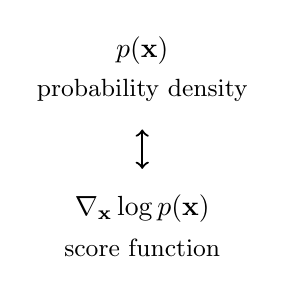
\begin{tikzpicture}
						\node at (0, 1) {$p(\mathbf{x})$};
						
						\node at (0, 0.5) {\small \text{probability density}};
						
						\draw[<->, thick] (0, 0) -- (0, -0.5);
						
						\node at (0, -1) {$\nabla_\mathbf{x} \log p(\mathbf{x})$};
						
						\node at (0, -1.5) {\small \text{score function}};
					\end{tikzpicture}
					
				\end{column}
				\begin{column}{0.5\textwidth}
					\begin{figure}
						\includegraphics[width=\textwidth]{CompareScoreFunction.png}
						\caption{\scriptsize score function vs probability density}
					\end{figure}
				\end{column}
			\end{columns}
		\end{column}
	\end{columns}	
\end{frame}




%	Ta gọi $\epsilon = \mathcal{N}(0, I)$
%\begin{columns}
%\begin{column}{0.8\textwidth}
%\begin{figure}
%	\centering
%	\includegraphics[width=\textwidth]{OverviewDiffusion}
%\end{figure}
%\end{column}
%
%\begin{column}{0.2\textwidth}
%
%\end{column}
%\end{columns}
%\\
%q(\mathbf{x}_t \vert \mathbf{x}_{t-1}) &= \mathcal{N}(\mathbf{x}_t; \sqrt{\alpha_t} \mathbf{x}_{t-1}, (1 - \alpha_t)\mathbf{I}) \\ 
%\rightarrow q(\mathbf{x}_t \vert \mathbf{x}_0) &= \mathcal{N}(\mathbf{x}_t; \sqrt{\bar{\alpha}_t} \mathbf{x}_0, (1 - \bar{\alpha}_t)\mathbf{I})



\section{Mô hình sinh cử chỉ}

%\begin{frame}{Tổng quan về bài toán}
%%	\begin{figure}
%%		\centering
%%		\includegraphics[width=0.8\linewidth]{SequenceGesture.jpg}
%%	\end{figure}
%%	
%	Cho chuỗi cử chỉ $\mathbf{g} \in \mathbb{R}^{(N+ M) \times D}$, với $\mathbf{s} \in \mathbb{R}^{N \times D}$ và đoạn cử chỉ nhãn $\mathbf{x}_0 \in \mathbb{R}^{M \times D}$ với $D=1141$, $N=8$, $M=80$. Chuỗi âm thanh $\mathbf{a} \in \mathbb{R}^{64000}$ (4s: $16000$ sample rate). Cảm xúc $\mathbf{e} \in \mathbb{R}^6$. 
%%	$\{\beta_t \in (0, 1)\}_{t=1}^T$
%
%\end{frame}


\begin{frame}{Diffusion cho bài toán sinh cử chỉ}
	\textbf{Điểm giống}
	\begin{itemize}
		\item Sử dụng mô hình Diffusion \cite{yang2023diffusestylegesture} trên cử chỉ $\bx^{1:M \times D}$,  với $M$ frame theo thời gian, $D=1141$ là các điểm toạ độ chuyển động của mỗi khung hình (tương tự width và height trong ảnh).
		\item Classifier-Free Diffusion Guidance với $\bx_0$ objective.
		\item Latent vector có số chiều là $256$.
		\end{itemize}
		
		\textbf{Điểm khác}
		
		\begin{itemize}
			\item Sinh cử chỉ có điều kiện:
			\begin{itemize}
				\item Điều kiện cảm xúc: $c = \big[ \mathbf{s}, \mathbf{e}, \mathbf{a} \big]$ và $c_{\varnothing} = \big[ \varnothing, \varnothing, \mathbf{a} \big]$.
				\item Nội suy trạng thái giữa hai cảm xúc $\mathbf{e}_1, \mathbf{e}_2$, sử dụng điều kiện: $c = \big[ \mathbf{s}, \mathbf{e}_1, \mathbf{a} \big]$ và $c_{\varnothing} = \big[ \mathbf{s}, \mathbf{e}_2, \mathbf{a} \big]$.
			\end{itemize}
			\item Self-Attention: Mối liên hệ giữa các cảm xúc, cử chỉ khởi tạo và từng frame (tương tự DALL-E 2 - mối liên hệ giữa văn bản và ảnh).
			\item Concat âm thanh (Giống ControlNet - Pixel-wise Condition)
%			\item Học mối liên hệ giữa điều kiện và các frame bằng Local-Cross Attention
		\end{itemize}
\end{frame}

\begin{frame}{Tổng quan các công đoạn}
	
	\begin{figure}
		\centering
		\includegraphics[width=\linewidth]{AllStage}
	\end{figure}
	
\end{frame}

\begin{frame}{Các công đoạn trong mô hình OHGesture}
	\begin{figure}
		\centering
		\includegraphics[width=\linewidth]{ModelStage}
	\end{figure}
\end{frame}

\begin{frame}{Diffusion cho bài toán sinh cử chỉ}
	
	\begin{figure}
		\centering
		\includegraphics[width=0.9\linewidth]{OverviewArchitecture.jpg}
	\end{figure}
	
\end{frame}

\begin{frame}{Kiến trúc OHGesture}
	\begin{figure}
		\centering
		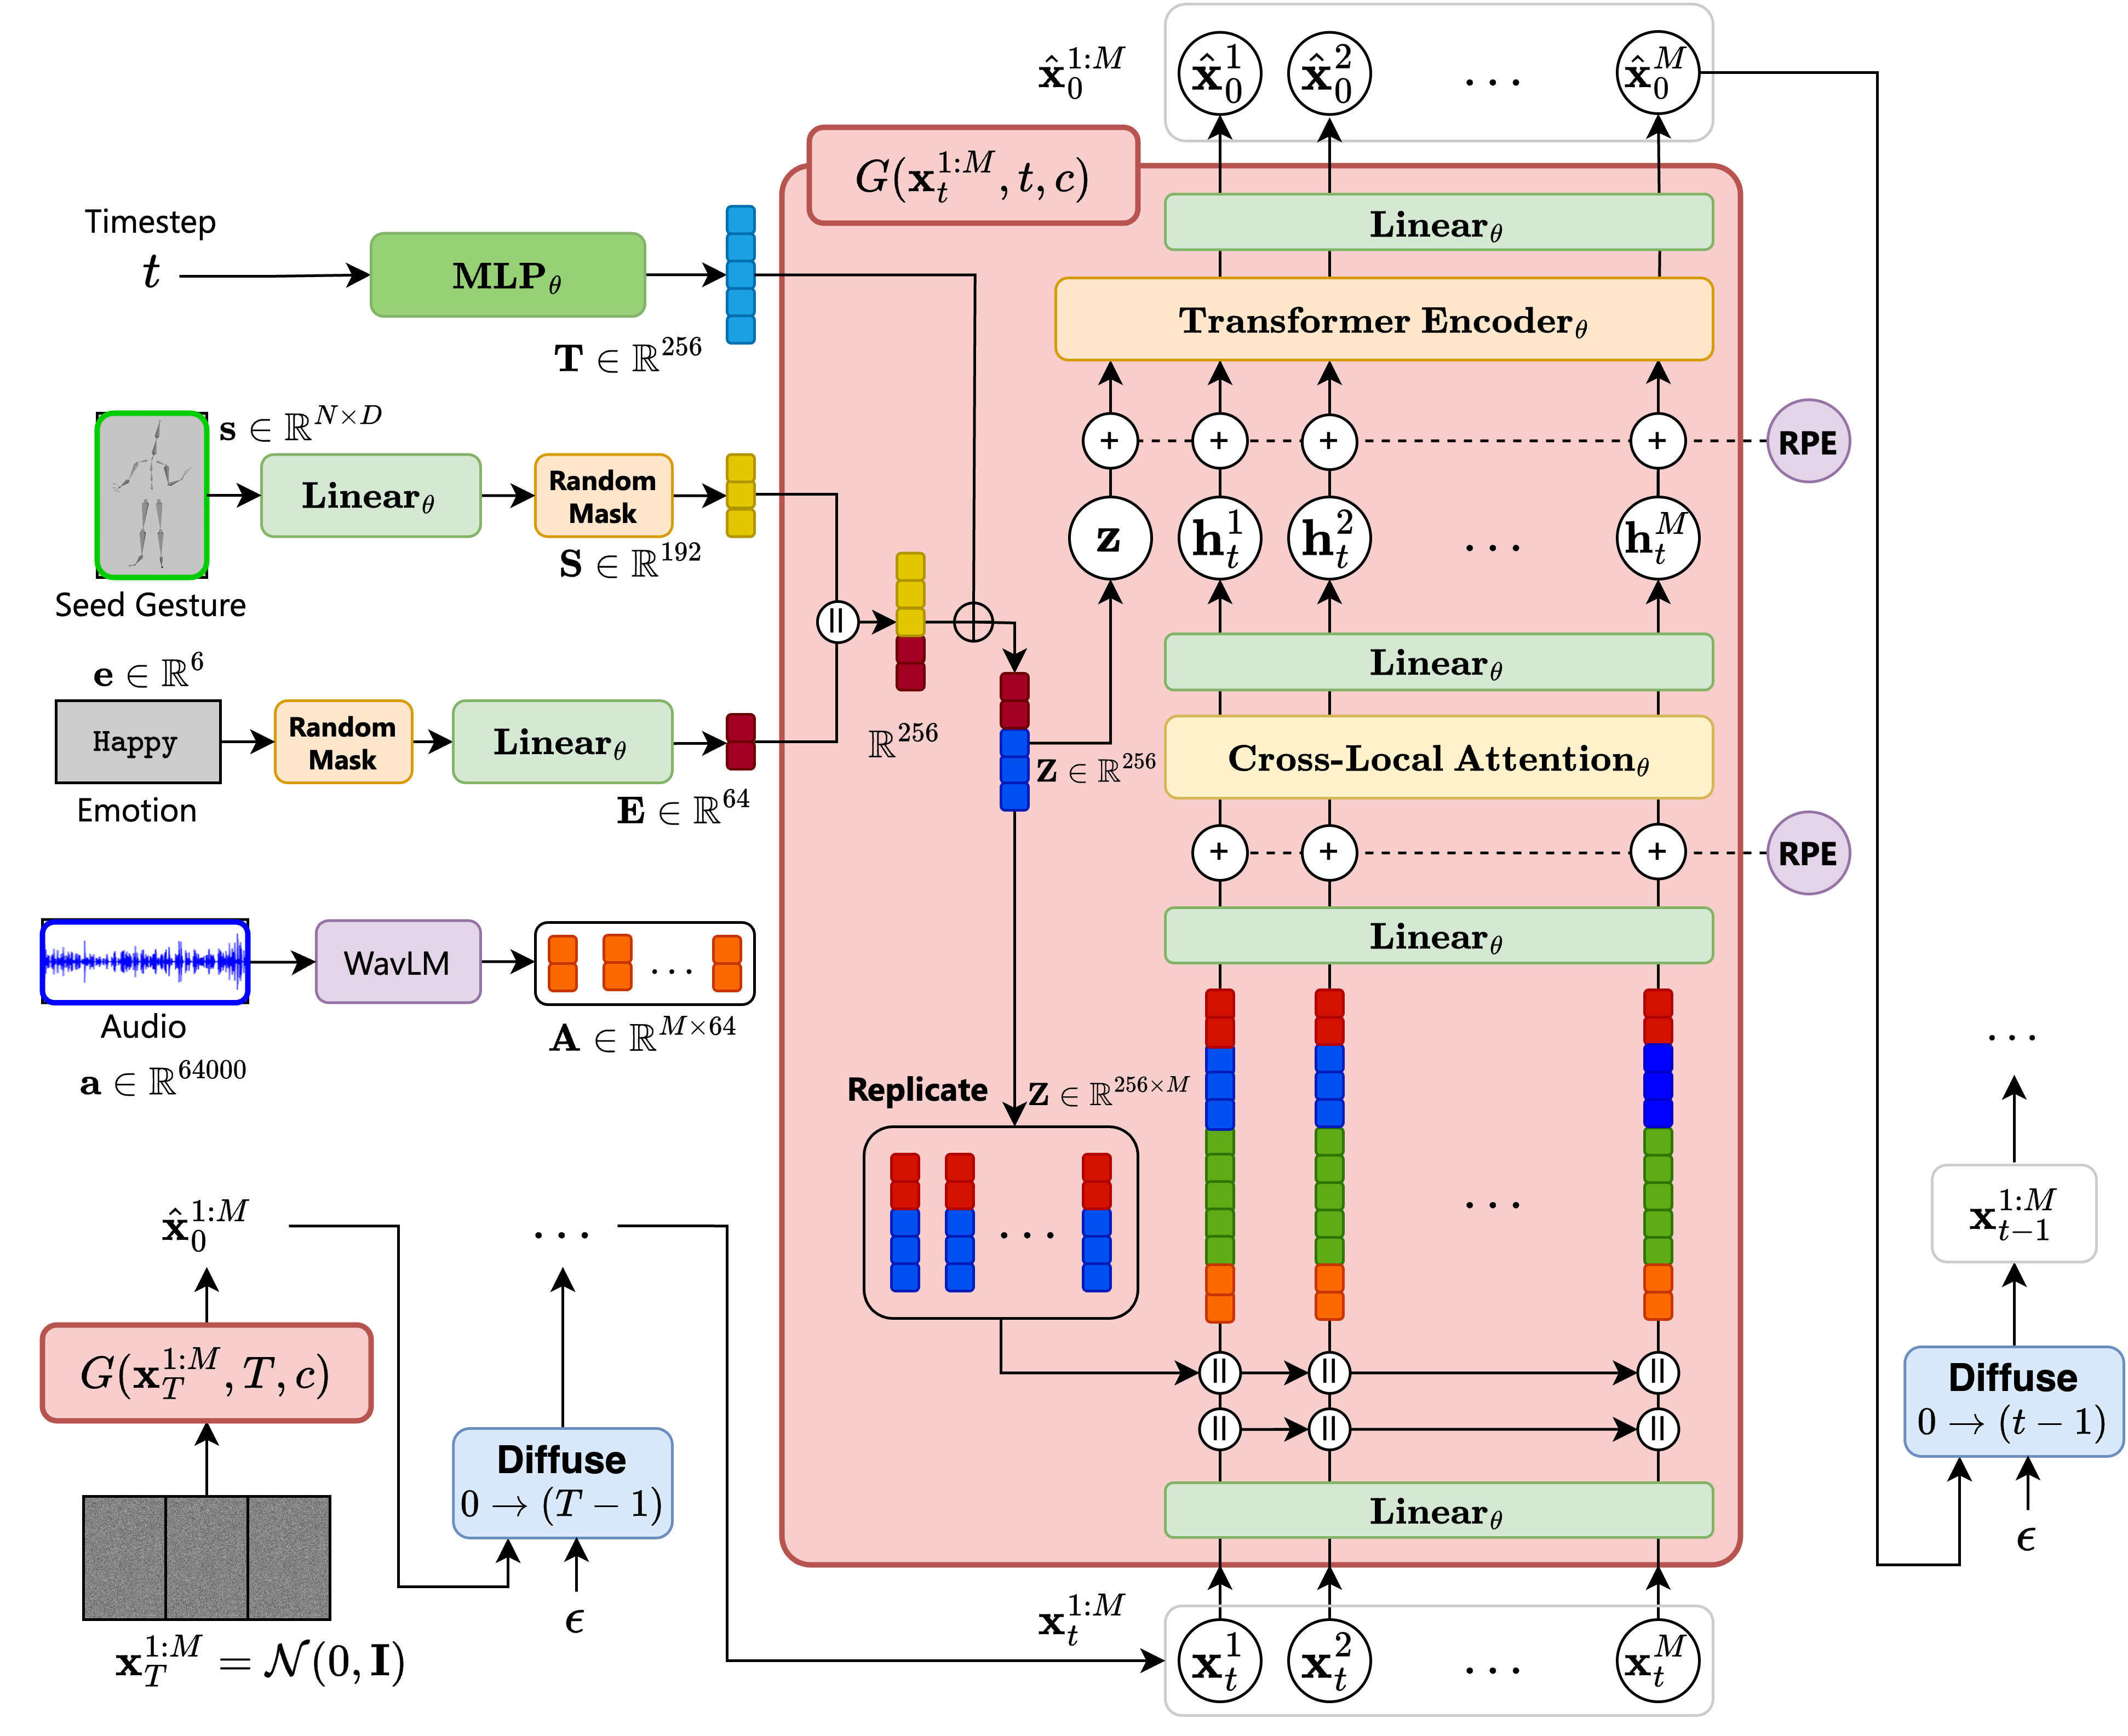
\includegraphics[width=0.9\linewidth]{OHGesture}
	\end{figure}
\end{frame}


\begin{frame}{Attention}
	\begin{figure}
		\centering
		\includegraphics[width=0.85\linewidth]{Attention}
	\end{figure}
\end{frame}

\begin{frame}{Cross-Local Attention and Self-Attention}
	\small
	\textbf{Cross-Local Attention}
	\begin{equation*} \label{eq:attention}
		\operatorname{Attention}(\mathbf{Q}, \mathbf{K}, \mathbf{V}, \mathbf{M})=\operatorname{softmax}\left(\frac{\mathbf{Q} \mathbf{K}^{T}+\mathbf{M}}{\sqrt{C}}\right) \mathbf{V}
	\end{equation*}
	

	\begin{columns}
%		Transfomer Encoder : 
		
		\begin{column}{0.5\textwidth}
				\textbf{Self-Attention}
			$$
			f_{\text{MultiHead}(\mathbf{X})} = \operatorname{concat} \left( \mathbf{H}_1, \mathbf{H}_2, \dots, \mathbf{H}_h \right) \mathbf{W}_O
			$$
			
			$$
			\mathbf{H}_i = \operatorname{softmax} \left( \frac{\mathbf{Q}_i \mathbf{K}_i^T}{\sqrt{d_k}} \right) \mathbf{V}_i
			$$
		\end{column}
		
		\begin{column}{0.5\textwidth}
			\begin{figure}
				\centering
				\includegraphics[width=\linewidth]{CrossLocalAttention}
			\end{figure}
		\end{column}
	\end{columns}

\end{frame}


%\begin{frame}
%	\begin{figure}
%		\centering
%		\includegraphics[width=0.8\linewidth]{DiffusionProcess}
%	\end{figure}
%\end{frame}


%\begin{figure} 
%	\centering
%	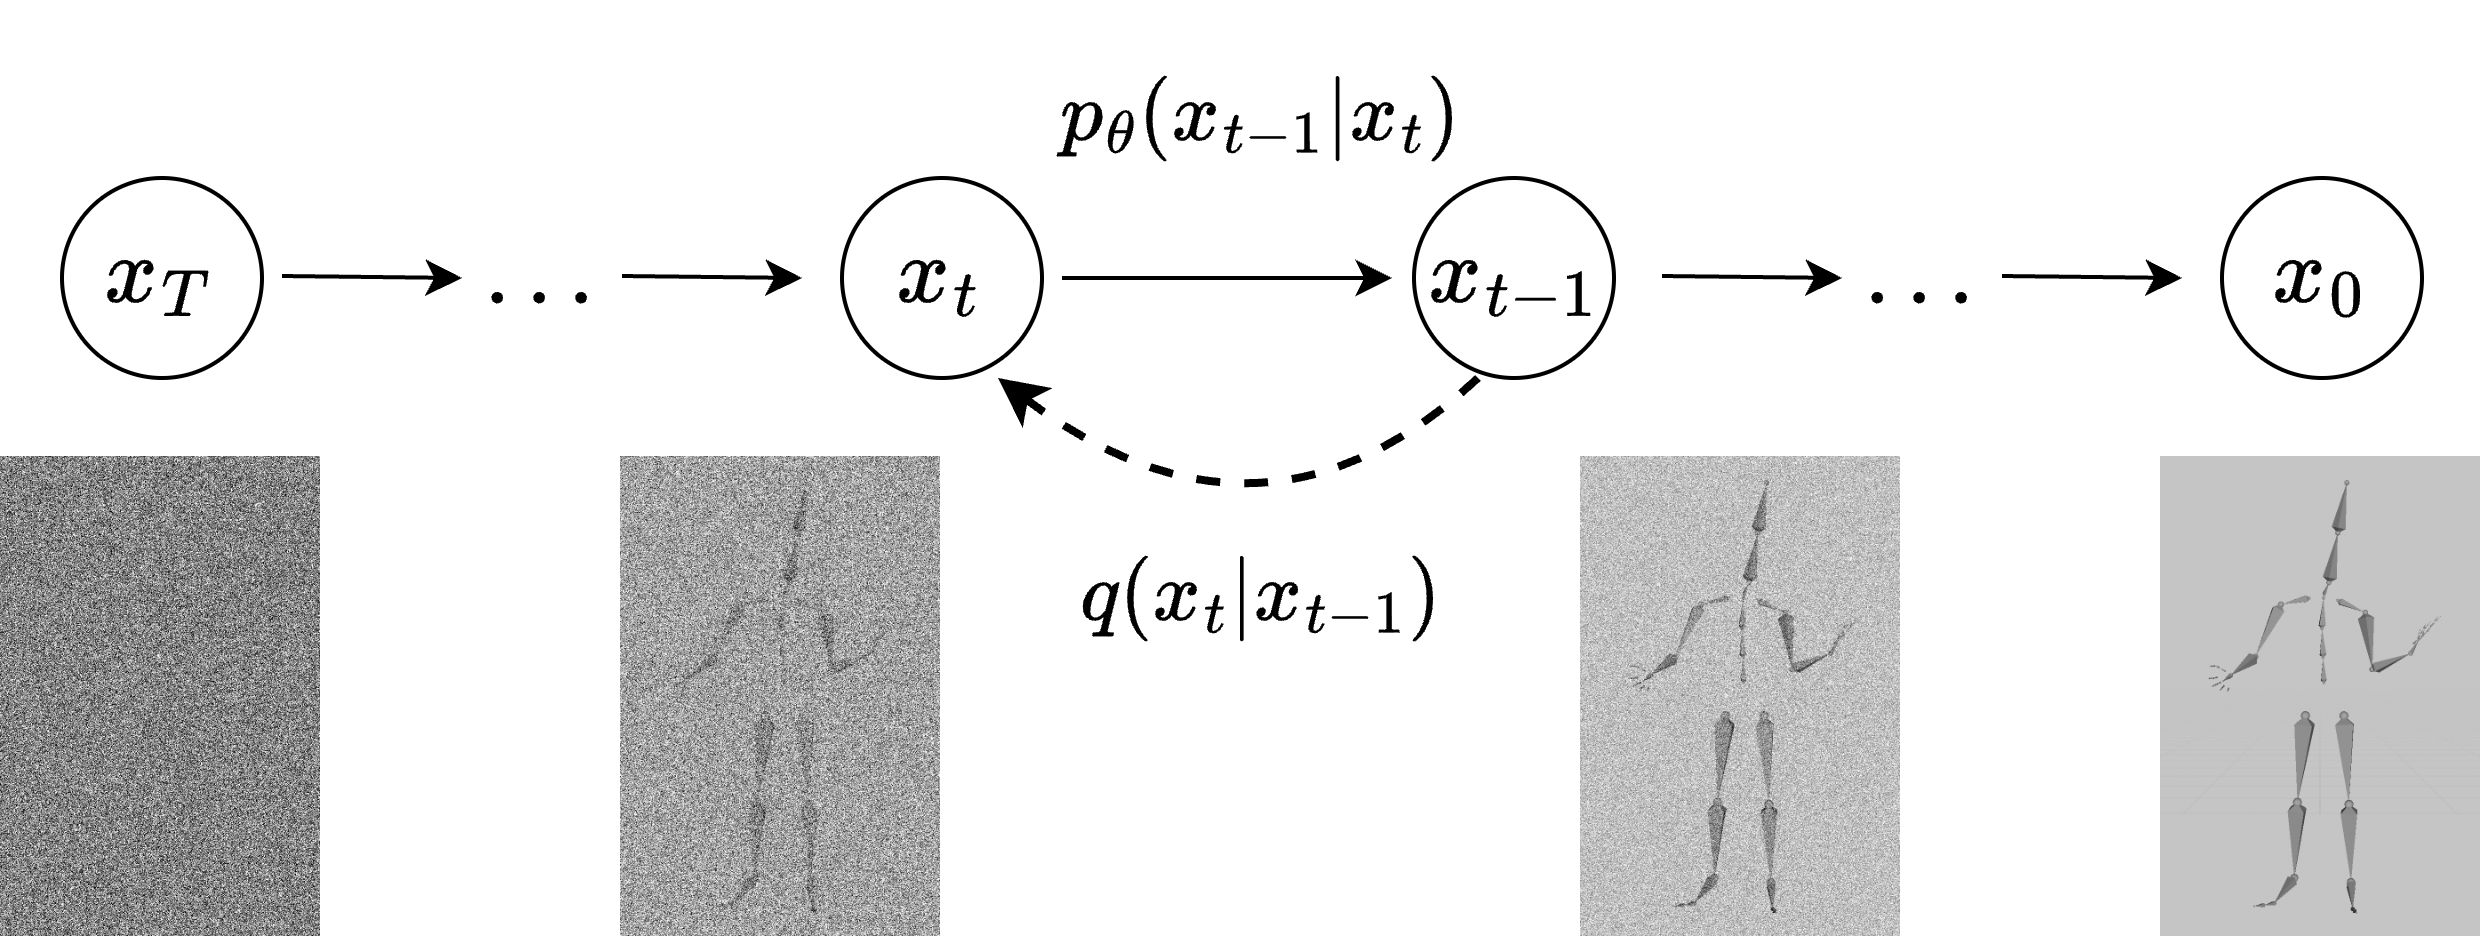
\includegraphics[width=0.8\linewidth]{DiffusionForward}
%\end{figure}


%\begin{frame}
%	
%	$
%	\label{Gaussian}
%	q\left(x_t \mid x_{t-1}\right)=\mathcal{N}\left(x_t ; \sqrt{1-\beta_t} x_{t-1}, \beta_t \mathbf{I}\right)
%	$
%	
%	$
%	\label{eq1}
%	q\left({x}_{1:T} \mid {x}_0\right)=\prod_{t=1}^T q\left({x}_t \mid {x}_{t-1}\right)
%	$
%	$
%	p_\theta\left({x}_{t-1} \mid {x}_t\right)=\mathcal{N}\left({x}_{t-1} ; {\mu}_\theta\left({x}_t, t\right), {\Sigma}_\theta\left({x}_t, t\right)\right)
%	$
%	
%	$
%	q\left({x}_t \mid {x}_0\right)=\mathcal{N}\left({x}_t ; \sqrt{\bar{\alpha}_t} {x}_0,\left(1-\bar{\alpha}_t\right) \mathbf{I}\right)
%	$
%	
%	$
%	\hat{x}_0=G\left(x_t, t, c\right)
%	$
%\end{frame}

	
%	\begin{columns}
	%		\begin{column}{0.5\textwidth}
		%			\textbf{DDPM (stochastic sampling):}
		%			\begin{itemize}
			%			\item Predict $x_0$ from $x_t$
			%			
			%			\item Convert to $\epsilon_{pred}$
			%			
			%			\item Use the formula:
			%			
			%			$$x_{t-1} = \frac{1}{\sqrt{\alpha_t}} x_t - \frac{1-\alpha_t}{\sqrt{1-\bar{\alpha}t}\sqrt{\alpha_t}} \epsilon_{\text{pred}} + \sigma_t z$$
			%			
			%			\item where $z \sim \mathcal{N}(0,I)$ is random noise
			%			\end{itemize}
		%			
		%		\end{column}
	%		
	%		\begin{column}{0.5\textwidth}
		%			\textbf{DDIM (deterministic sampling):}
		%			
		%			Predict $x_0$ from $x_t$
		%			
		%			NO additional noise term ($\sigma_t = 0$)
		%			
		%			Use the formula:
		%			
		%			$x_{t-1} = \sqrt{\bar{\alpha}{t-1}} x_0^{\text{pred}} + \sqrt{1-\bar{\alpha}_{t-1}} \epsilon_{\text{pred}}$
		%			
		%			Where:
		%			\begin{itemize}
			%			\item $\bar{\alpha}_t$ is the cumulative product of $\alpha$'s from 1 to t
			%			\item $\epsilon_{pred}$ is derived from $x_0$ prediction using:
			%			\item $\epsilon_{pred} = \frac{x_t - \sqrt{\alpha_t}x_{0_{pred}}}{\sqrt{1-\alpha_t}}$
			%			\end{itemize}
		%		\end{column}
	%	\end{columns}
	


%
\section{Thực nghiệm}

\begin{frame}{Dataset}
	
%	$x^{2} \in \mathbb{R}^{x \times y}$

\begin{columns}
	\begin{column}{0.5\textwidth}
		ZeroEGGs Dataset
		\begin{itemize}
			\item Happy,  Sad, Neutral
			\item Old, Relaxed, Angry
		\end{itemize}
		%	\includepdf[pages=-]{images/EmotionPCA.pdf}
		\includegraphics[width=\linewidth]{EmotionPCA.pdf}
	\end{column}
	
	\begin{column}{0.5\textwidth}
		\includegraphics[width=\linewidth]{ZEGGsData}
	\end{column}
\end{columns}
\end{frame}

%\begin{frame}{Training Process}
%
%\end{frame}


%

\begin{frame}{Độ đo}
	Các độ đo trong Gesture Generation:
	\begin{itemize}
		\item Human-likeness 
		\item Gesture-Speech Appropriateness
		\item Gesture-style Appropriateness
	\item {FID (Fréchet Inception Distance)}:
%	\vspace{-5mm}
	\begin{equation*}
		\operatorname{FID} = \left\| \mu_{\operatorname{real}} - \mu_{\operatorname{fake}} \right\|^2 + \operatorname{Tr} \left( \Sigma_{\operatorname{real}} + \Sigma_{\operatorname{fake}} - 2 \left( \Sigma_{\operatorname{real}} \Sigma_{\operatorname{fake}} \right)^{\frac{1}{2}} \right)
	\end{equation*}
%	\vspace{-5mm}
	 \item Mean opinion scores (MOS)
	
\end{itemize}
\end{frame}
\begin{frame}{Kết quả}
	\begin{columns}
	\begin{column}{0.33\textwidth}
		\includegraphics[width=\linewidth]{BoxHumanLikeness.pdf}
	\end{column}
	
	\begin{column}{0.33\textwidth}
		\includegraphics[width=\linewidth]{BoxSpeechAppropriateness.pdf}
	\end{column}
	
	\begin{column}{0.33\textwidth}
		\includegraphics[width=\linewidth]{BoxStyleAppropriateness.pdf}
	\end{column}
\end{columns}

%Thử nghiệm với các thành phần cấu trúc trong mô hình:	
%
%\begin{enumerate}
%\item Sử dụng đặc trưng WavLM
%\item 
%\end{enumerate}

%\begin{itemize}
%	\item (1)sdf 
%\end{itemize}

\begin{table}[!t]
%	\footnotesize
\tiny
	\centering
	\resizebox{\columnwidth}{!}{%
		\begin{tabular}{lcc}
			\hline
			\multicolumn{1}{c}{Name} &
			\begin{tabular}[c]{@{}c@{}}Human\\ likeness \end{tabular}$\uparrow$ &
			\begin{tabular}[c]{@{}c@{}}Gesture-speech\\ appropriateness\end{tabular}$\uparrow$ \\ \hline
			Ground Truth          & 4.15 $\pm$ 0.11          & 4.25 $\pm$ 0.09          \\
			Ours                  & \textbf{4.11 $\pm$ 0.08} & \textbf{4.11 $\pm$ 0.10} \\
			\quad$-$ WavLM             & 4.05 $\pm$ 0.10          & 3.91 $\pm$ 0.11          \\
			\quad$-$ Cross-local attention   & 3.76 $\pm$ 0.09          & 3.51 $\pm$ 0.15          \\
			\quad$-$ Self-attention    & 3.55 $\pm$ 0.13          & 3.08 $\pm$ 0.10          \\
			% \begin{tabular}[c]{@{}c@{}}$-$ attention (GRU based) \\ (GRU based)\end{tabular} &
			\quad$-$ Attention + GRU&
			3.10 $\pm$ 0.11 &
			2.98 $\pm$ 0.14 \\
			\quad$+$ Forward attention & 3.75 $\pm$ 0.15          & 3.23 $\pm$ 0.24          \\
			\hline
		\end{tabular}%
	}
%	\caption{Kết quả của các nghiên cứu loại bỏ (Ablation studies). "$-$" chỉ các mô-đun không được sử dụng và "$+$" chỉ các mô-đun bổ sung. Chữ in đậm chỉ ra chỉ số tốt nhất.}
	\label{Ab}
\end{table}

\end{frame}


%
\section{Kết luận}

\begin{frame}{Giải quyết các thách thức}
		\begin{itemize}
			\item Bằng việc dùng Cross-Local Attention và Self-Attention, chúng tôi giải quyết được quan hệ $1:n$ của cử chỉ và các điều kiện âm thanh, cảm xúc.
			\item Mô hình Diffusion giúp mô hình có thể học được các đặc trưng có phân bố dữ liệu thật thấp.
			\item Đảm bảo khả năng mở rộng (scalable) của hệ thống sinh cử chỉ để có thể ứng dụng trong thực tế.
		\end{itemize}
\end{frame}

\begin{frame}{Đóng góp chính}
	
	\begin{figure}
		\centering
		\includegraphics[width=0.9\linewidth]{TotalStage}
	\end{figure}
	
	\begin{itemize}
		\item Transcribe âm thanh để có được văn bản (\textit{Công đoạn tiền xử lý}, \textit{xử lý đặc trưng} và \textit{kết hợp đặc trưng}), làm dữ liệu bổ sung trong Diffusion có điều kiện.
		
		\item Mở rộng mã nguồn chương trình: \hyperlink{https://github.com/hmthanh/OHGesture}{\textbf{github.com/OHGesture}}, Mô hình pretrain: \hyperlink{https://huggingface.co/openhuman/openhuman}{\textbf{Huggingface.co/openhuman}}
		
		\item Giai đoạn Hệ thống trực quan hoá bằng Unity (\textit{Công đoạn Kết xuất}): \hyperlink{https://github.com/DeepGesture/deepgesture-unity}{\textbf{github.com/DeepGesture-Unity}}.
		
		\item Genea Leaderboard: Paper xây dựng hệ thống chuẩn hoá
		
		\item Đánh giá cử chỉ bằng FID: \hyperlink{https://github.com/GestureScore/GestureScore}{\textbf{github.com/GestureScore}}.
	\end{itemize}
\end{frame}

\begin{frame}[label=frame]{{Kết luận}}
	\begin{itemize}
		\item Mô hình \textbf{OHGesture}, có khả năng sinh cử chỉ chân thực, không chỉ trên các mẫu dữ liệu trong tập huấn luyện mà còn mở rộng được với những âm thanh không có trong dữ liệu huấn luyện.
		
		\item Sử dụng phương pháp \textbf{Classifier-free Guidance}, có thể điều khiển các điều kiện như cảm xúc, cử chỉ khởi tạo, có thể nội suy để suy luận ra giữa các cảm xúc khác nhau.
		
		\item Bài toán sinh cử chỉ còn rất mới, chúng tôi dự định sẽ dùng Fourier TT để trích xuất các đặc trưng về pha.
		
	\end{itemize}
	

%	In this slide, some important text will be
%	\alert{highlighted} because it's important.
%	Please, don't abuse it.
%	
%	\begin{block}{Remark}
%		Sample text
%	\end{block}
%	
%	\begin{alertblock}{Important theorem}
%		Sample text in red box
%	\end{alertblock}
%	
%	\begin{examples}
%		Sample text in green box. The title of the block is ``Examples".
%	\end{examples}
%	\hyperlink{appendix}{\beamerbutton{More on Appendix}}
\end{frame}

%

%\begin{frame}{Reference 2 s}
%	\cite{yang2023diffusestylegesture}
%\end{frame}


\begin{frame}[allowframebreaks]{References}
	
	{\footnotesize
    \printbibliography}
\end{frame}


\end{document}

